%% LyX 2.2.1 created this file.  For more info, see http://www.lyx.org/.
%% Do not edit unless you really know what you are doing.
%\documentclass[english]{article}
%\usepackage[latin9]{inputenc}

%\usepackage{babel}
%begin{document}

\documentclass[english]{article}
\usepackage[T1]{fontenc}
\usepackage[latin9]{inputenc}
\usepackage[a4paper]{geometry}
\usepackage{amsmath}
\geometry{verbose,tmargin=2cm,bmargin=2cm,lmargin=2cm,rmargin=2cm}
\usepackage{graphicx}
%\usepackage[chapter]{algorithm}
\usepackage{algorithmic}
\newcommand{\norm}[1]{\left\lVert#1\right\rVert}

\DeclareMathOperator*{\argmin}{\arg\!\min}
\DeclareMathOperator*{\argmax}{\arg\!\max}

\makeatletter

%%%%%%%%%%%%%%%%%%%%%%%%%%%%%% LyX specific LaTeX commands.
%% Because html converters don't know tabularnewline
\providecommand{\tabularnewline}{\\}

\makeatother

\usepackage{babel}
\begin{document}

\title{Machine Learning for Computer Vision (EE5177) \\ Programming Assignment 3 : Regression Models \\ Problem \#1}

\author{Akshit Kumar \\ \emph{EE14B127}}

\date{29th March 2017}

\maketitle
\tableofcontents{}

\section{Introduction}

\subsection{Goal}
The first problem of the programming assignment requires us to use non linear regression to fit a $sinc$ function (non-linear curve) using an RBF kernel and arctan kernel. 

\subsection{Approach}
To fit a non-linear function, we first generate our ground truth data by setting the world states to $sinc(x)$, in order the generate synthetic data for curve fitting, we add noise to the ground truth data and use RBF kernel and arctan kernel to fit the data to it. 

\subsection{Results}
The number of kernels is initially taken to be 7. The number of kernels can be varied to minimise the error. It can be noticed that beyond a certain number of kernels, the error does not decrease.

\section{Data Generation}
\subsection{Plot of $x$ vs. $y$ (Ground Truth Data)}
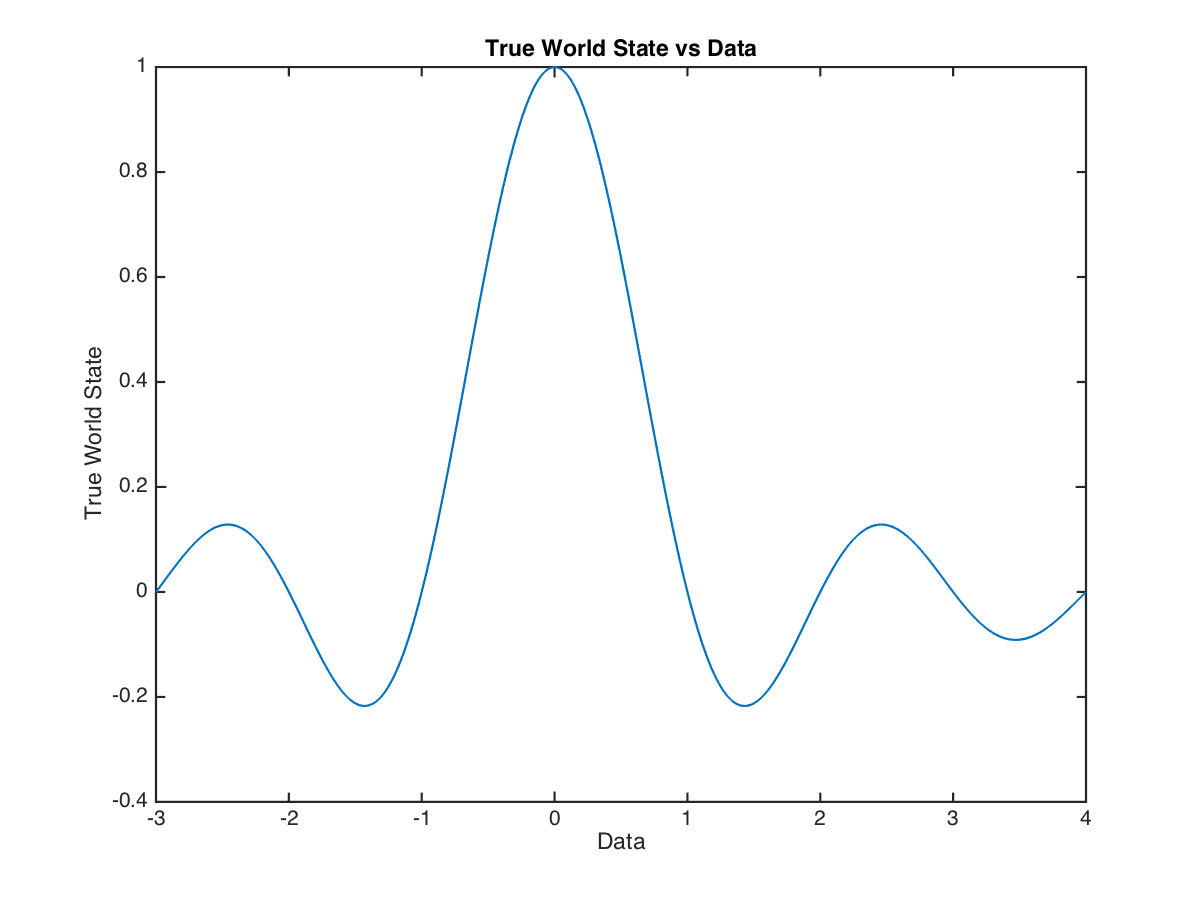
\includegraphics[scale=0.5]{../plots/sinc}

\subsection{Plot of $x$ vs. $w$}
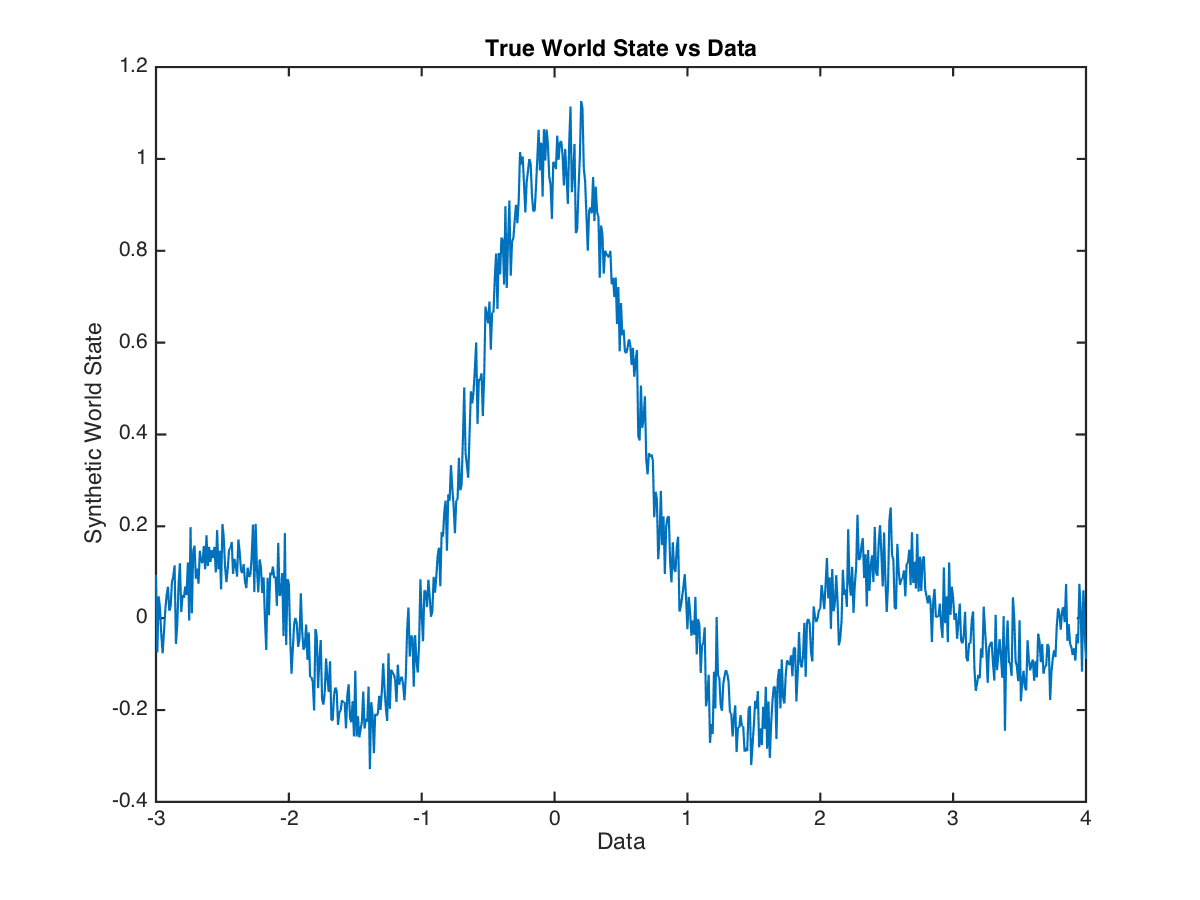
\includegraphics[scale=0.5]{../plots/sinc_noise}

\subsection{Rational for using non linear regression}
The relationship between the world states w and the input data x is not linear (sinc is not a linear function). Therefore we transform our input data through a nonlinear transformation as we would like to retain the mathematical convenience of the linear model while extending the class of functions that can be described.

\section{Non Linear Regression using Radial Basis Function (Gaussian)}
\subsection{Transformation Equation}
The input data x is transformed using the non linear function given by 
$$ z_i = f[x_i] $$
$$z_i=\begin{bmatrix}
1\\
exp[-(x_i-\alpha_1)^2/\lambda]\\
exp[-(x_i-\alpha_2)^2/\lambda]\\
exp[-(x_i-\alpha_3)^2/\lambda]\\
exp[-(x_i-\alpha_4)^2/\lambda]\\
exp[-(x_i-\alpha_5)^2/\lambda]\\
exp[-(x_i-\alpha_6)^2/\lambda]
\end{bmatrix} $$

\subsection{Choice of $\alpha$'s}
The $\alpha$s are chosen as means of the intervals, partitioning the dataset into appropriate number of intervals depending upon the number of kernel functions to be used.

\subsection{Choice of $\lambda$}
The value of $\lambda$ is initially arbitarily chosen to be 1 and then varied from 0.01 to 7 in steps on 0.001 and optimal $\lambda$ value is found which minimizes the prediction error and fitting error.

\subsection{Weight Estimation using MLE}
The optimal weights can be computed using
$$ \phi = (ZZ^{T})^{-1}Zw $$ where the matrix $Z$ contains the transformed vectors $\{z_i\}_{i=1}^{I}$ in its columns.

\subsection{World State Estimation (using $\lambda$ = 1)}
\subsubsection{Plot of the Predicted World State vs Data}
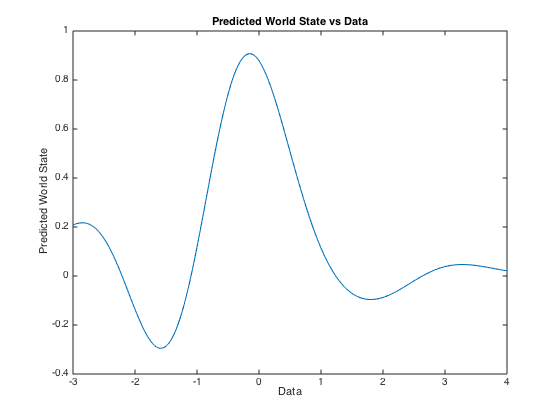
\includegraphics[scale=0.5]{../plots/pred_world_state_rbf}
\subsubsection{Prediction and Fitting Error}
Prediction Error = \textbf{\emph{0.1137}} 
\newline
Fitting Error = \textbf{\emph{0.1255}}

\subsection{Error Analysis}
\subsubsection{Prediction Error}
Predicition Error is the RMSE between the estimate of the weights and the ground truth value. It can be defined as 
$$ P.E = \norm{\phi^{T}z - y}_{2} $$

\subsubsection{Fitting Error}
Fitting Error is the RMSE between the estimate of the weights and the noisy data sample. It can be defined as 
$$ P.E = \norm{\phi^{T}z - w}_{2} $$

\subsection{Varying $\lambda$}
\subsubsection{Plot of Prediction Error}
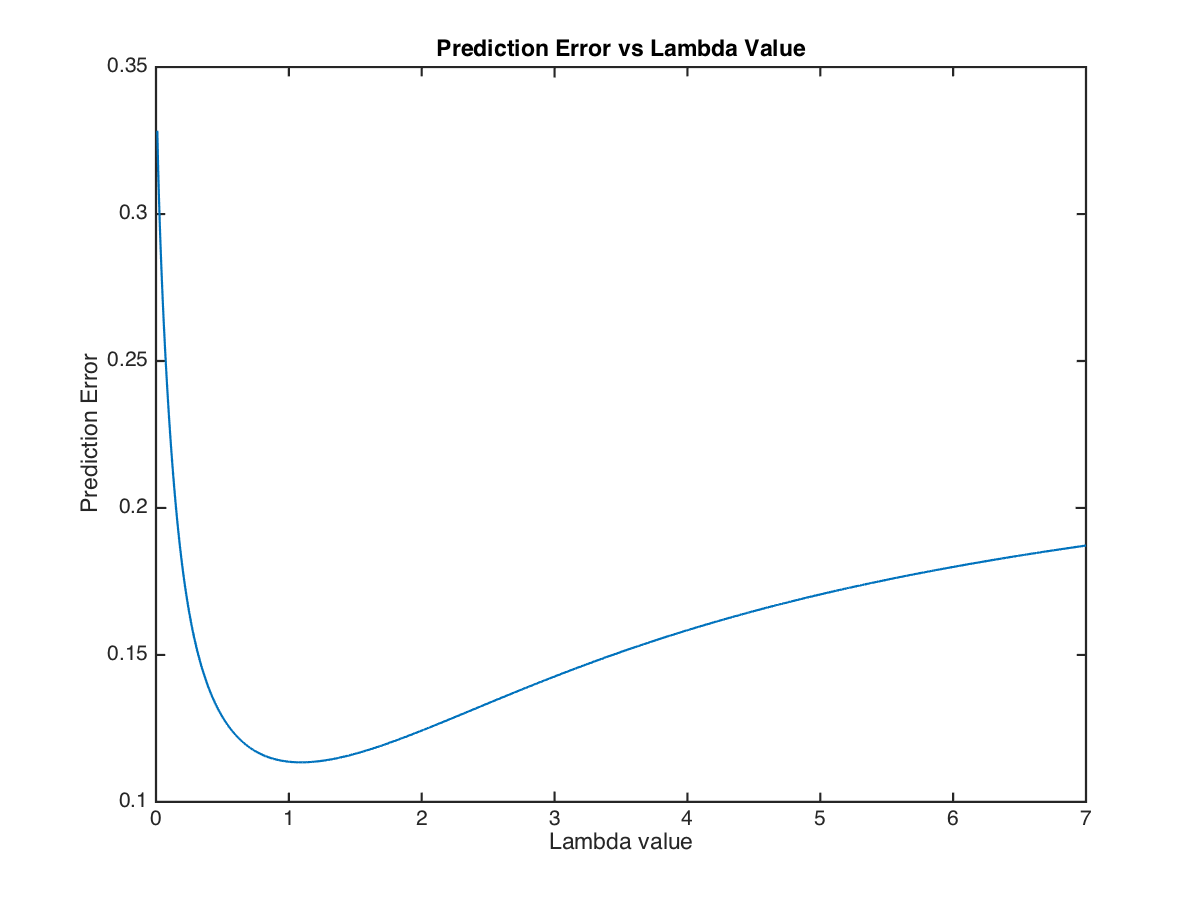
\includegraphics[scale=0.5]{../plots/pred_error_vs_lambda_rbf}
\subsubsection{Plot of Fitting Error}
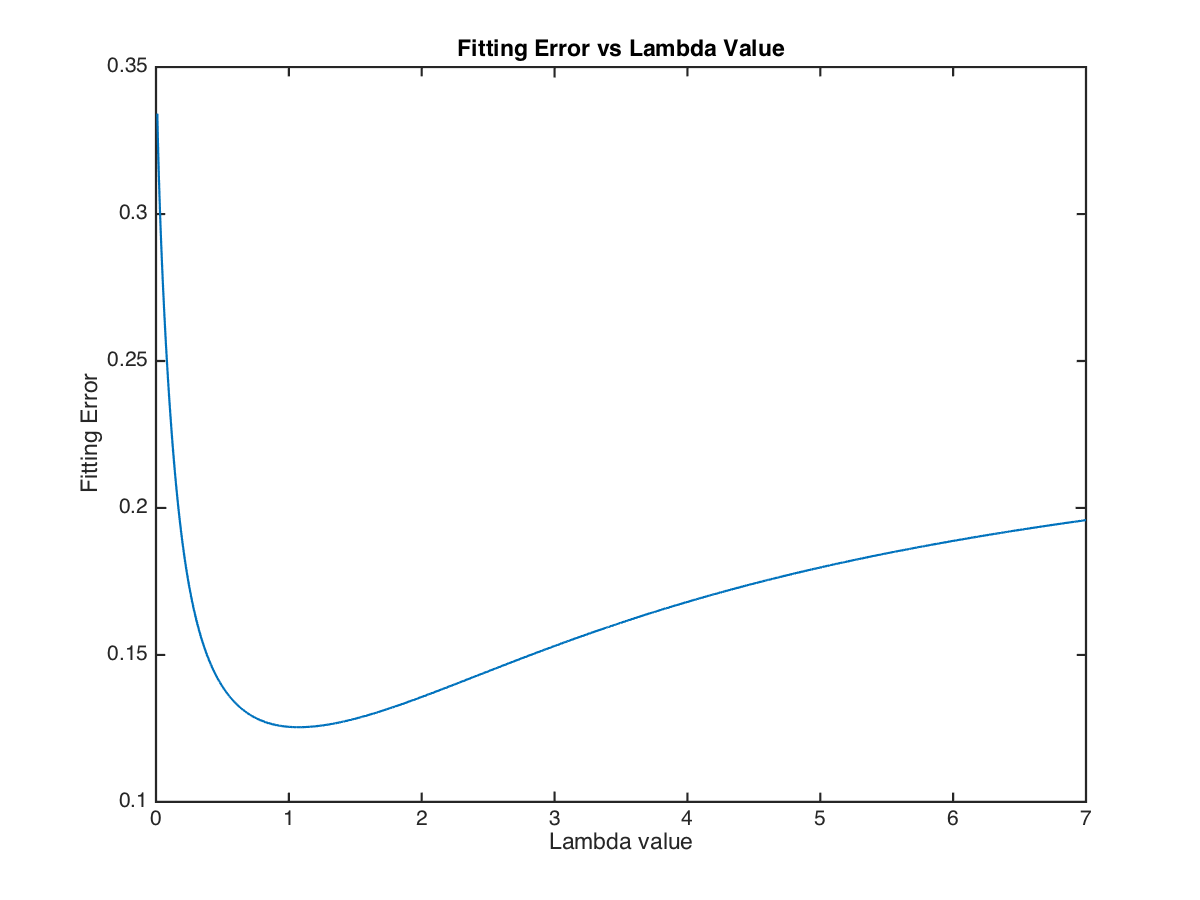
\includegraphics[scale=0.5]{../plots/fit_error_vs_lambda_rbf}
\subsubsection{Results}
The value of $\lambda$ corresponding to the minimum prediction error is \textbf{\emph{1.0910}}.
\newline
The minimum prediction error is \textbf{\emph{0.1135}}.
\newline
The value of $\lambda$ corresponding to the minimum fitting error is \textbf{\emph{1.0750}}. Note, this is not a deterministic value as it depends on the noisy-ness of the data.
\newline
The minimum fitting error is \textbf{\emph{0.1254}}.
\subsubsection{Explanation}
For small values of $\lambda$ the error decreases rapidly. For some value of $\lambda$ the error hits the minimum and then continues to increase. $\lambda$ represents an estimate of the variance of the data around the peaks given by $\alpha$'s. Once we get to the required variance by iterating through the different values of $\lambda$, we get the best prediction of the data and hence the least error.

\subsection{Varying the number of kernels}
\subsubsection{Plot of Prediction Error}
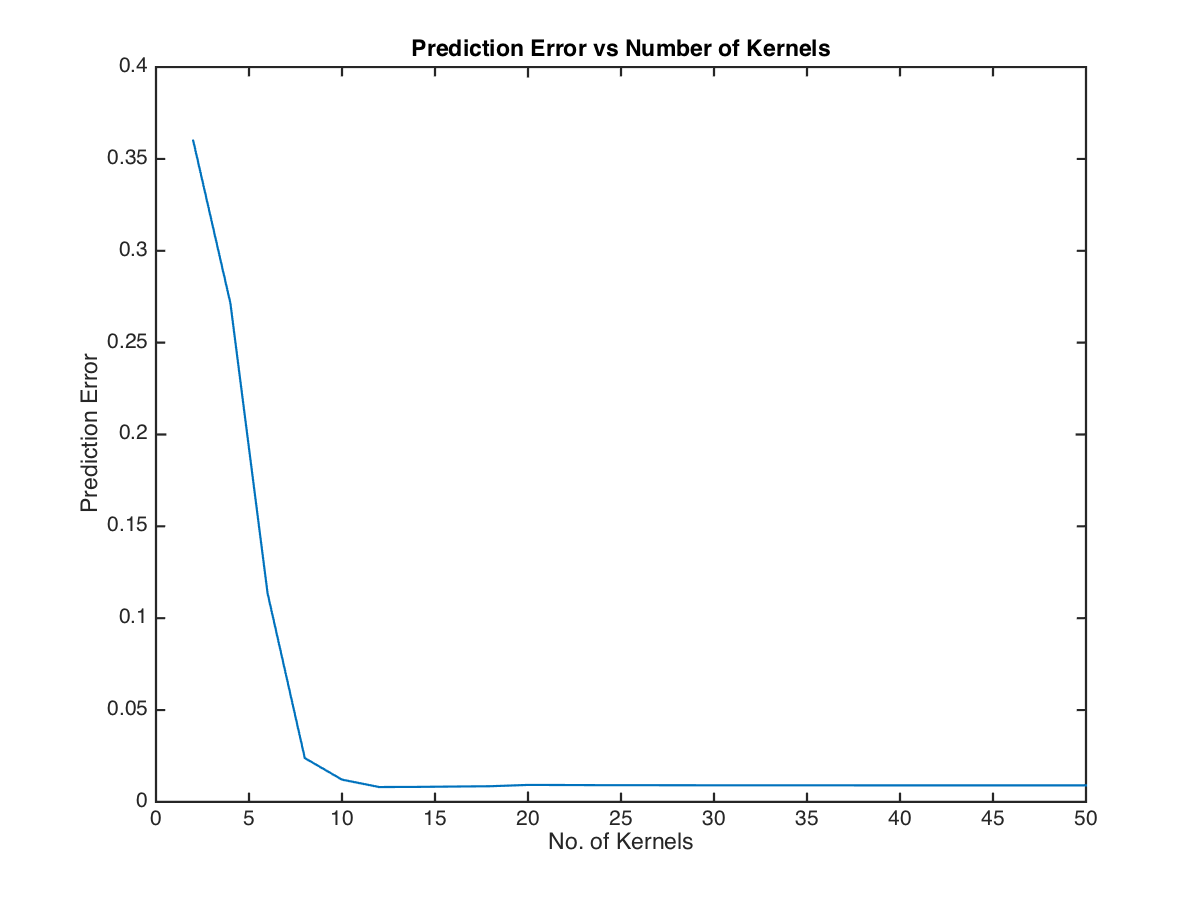
\includegraphics[scale=0.5]{../plots/pred_error_vs_num_kernels}
\subsubsection{Optimal number of kernel functions}
The optimal number of kernel functions obtained is \textbf{{\emph{14}}} with $\lambda = 1.0910$
\subsubsection{Explanation}
Getting the number of kernels required for minimum prediction error implies that 14 components are sufficient for explaining the data and better compared to the use of a larger number of components. Thus adding more degrees of freedom to the vector $\phi$ is not going to improve the estimation and reduce the prediction error.

\section{Non Linear Regression using Sigmoid function(Arc tangent)}
\subsection{Transformation Equation}
The input data x is transformed using the non linear function given by 
$$ z_i = f[x_i] $$
$$z_i=\begin{bmatrix}
exp[-(\lambda x_i-\alpha_1)]\\
exp[-(\lambda x_i-\alpha_2)]\\
exp[-(\lambda x_i-\alpha_3)]\\
exp[-(\lambda x_i-\alpha_4)]\\
exp[-(\lambda x_i-\alpha_5)]\\
exp[-(\lambda x_i-\alpha_6)]\\
exp[-(\lambda x_i-\alpha_7)]
\end{bmatrix}$$

\subsection{Choice of $\alpha$'s}
The $\alpha$s are chosen as means of the intervals, partitioning the dataset into appropriate number of intervals depending upon the number of kernel functions to be used.

\subsection{Choice of $\lambda$}
The value of $\lambda$ is initially arbitarily chosen to be 1 and then varied from 0.01 to 7 in steps on 0.001 and optimal $\lambda$ value is found which minimizes the prediction error and fitting error.

\subsection{Weight Estimation using MLE}
The optimal weights can be computed using
$$ \phi = (ZZ^{T})^{-1}Zw $$ where the matrix $Z$ contains the transformed vectors $\{z_i\}_{i=1}^{I}$ in its columns.

\subsection{World State Estimation (using $\lambda$ = 1)}
\subsubsection{Plot of the Predicted World State vs Data}
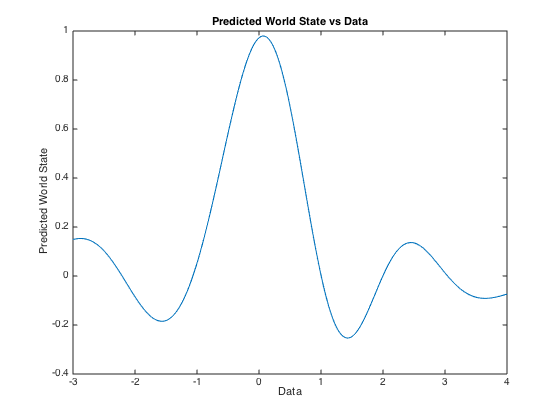
\includegraphics[scale=0.5]{../plots/pred_world_state_arctan}
\subsubsection{Prediction and Fitting Error}
Prediction Error = \textbf{\emph{0.0457}} 
\newline
Fitting Error = \textbf{\emph{0.0718}}

\subsection{Error Analysis}
\subsubsection{Prediction Error}
Predicition Error is the RMSE between the estimate of the weights and the ground truth value. It can be defined as 
$$ P.E = \norm{\phi^{T}z - y}_{2} $$

\subsubsection{Fitting Error}
Fitting Error is the RMSE between the estimate of the weights and the noisy data sample. It can be defined as 
$$ P.E = \norm{\phi^{T}z - w}_{2} $$

\subsection{Varying $\lambda$}
\subsubsection{Plot of Prediction Error}
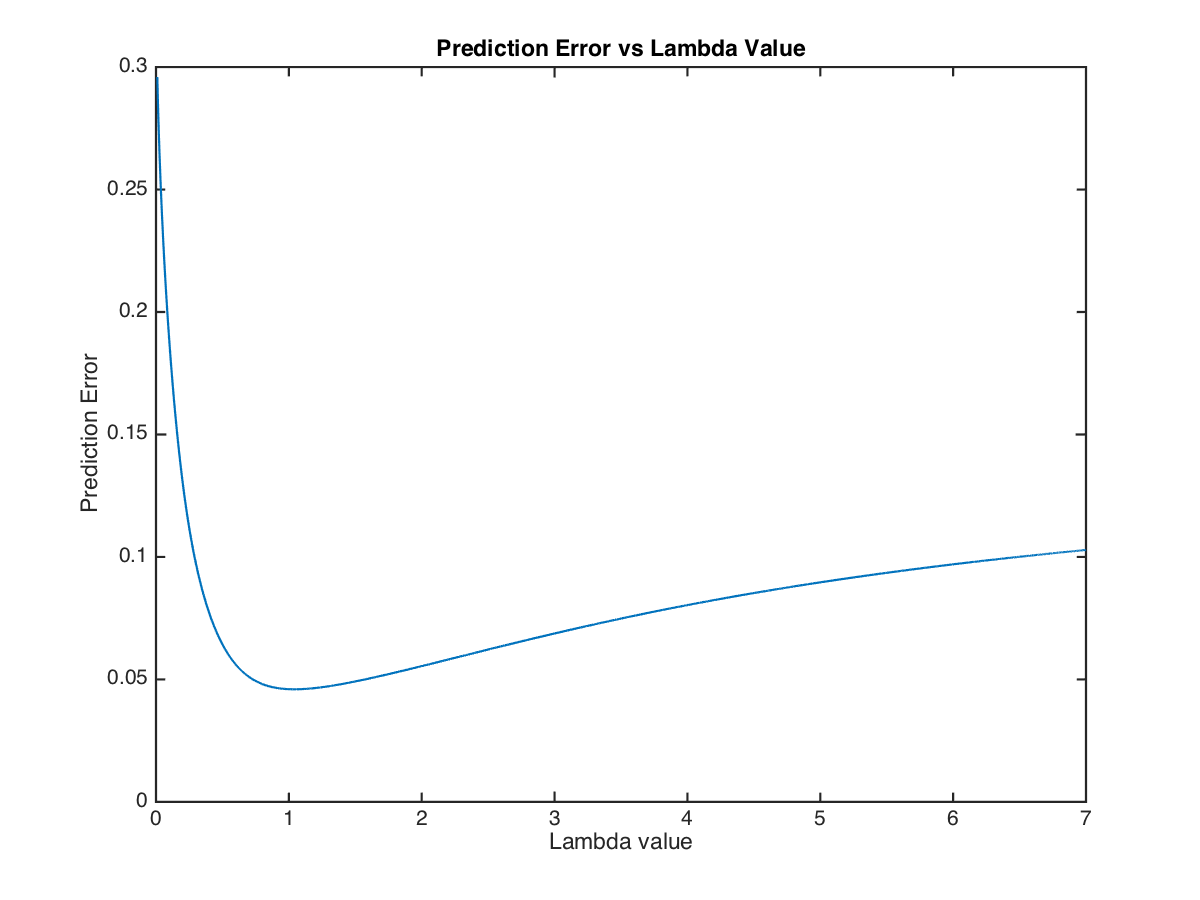
\includegraphics[scale=0.5]{../plots/pred_error_vs_lambda_arctan}
\subsubsection{Plot of Fitting Error}
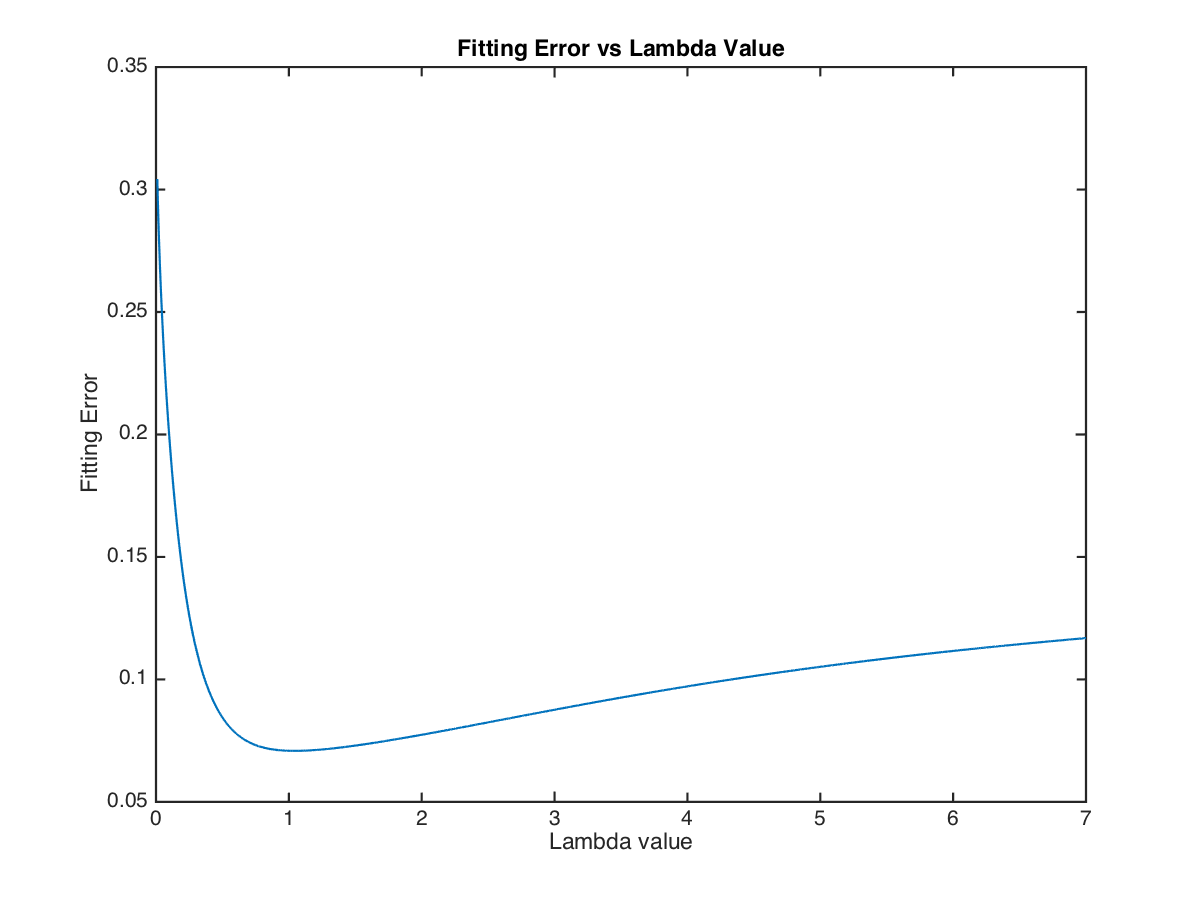
\includegraphics[scale=0.5]{../plots/fit_error_vs_lambda_arctan}
\subsubsection{Results}
The value of $\lambda$ corresponding to the minimum prediction error is \textbf{\emph{1.0410}}.
\newline
The minimum prediction error is \textbf{\emph{0.0456}}.
\newline
The value of $\lambda$ corresponding to the minimum fitting error is \textbf{\emph{1.0430}}. Note, this is not a deterministic value as it depends on the noisy-ness of the data.
\newline
The minimum fitting error is \textbf{\emph{0.0718}}.
\subsubsection{Explanation}
For small values of $\lambda$ the error decreases rapidly. For some value of $\lambda$ the error hits the minimum and then continues to increase. $\lambda$ represents an estimate of the variance of the data around the peaks given by $\alpha$'s. Once we get to the required variance by iterating through the different values of $\lambda$, we get the best prediction of the data and hence the least error.





\end{document}
